\documentclass[a4paper,UTF8]{article}
\usepackage{ctex}
\usepackage[margin=1.25in]{geometry}
\usepackage{color}
\usepackage{graphicx}
\usepackage{amssymb}
\usepackage{amsmath}
\usepackage{amsthm}
\usepackage{enumerate}
\usepackage{bm}
\usepackage{hyperref}
\usepackage{pgfplots}
\usepackage{epsfig}
\usepackage{color}
\usepackage{mdframed}
\usepackage{lipsum}
\newmdtheoremenv{thm-box}{myThm}
\newmdtheoremenv{prop-box}{Proposition}
\newmdtheoremenv{def-box}{定义}
\newmdtheoremenv{theorem}{定理}

\usepackage{listings}
\usepackage{xcolor}
\lstset{
	numbers=left, 
	numberstyle= \tiny, 
	keywordstyle= \color{ blue!70},
	commentstyle= \color{red!50!green!50!blue!50}, 
	frame=shadowbox, % 阴影效果
	rulesepcolor= \color{ red!20!green!20!blue!20} ,
	escapeinside=``, % 英文分号中可写入中文
	xleftmargin=2em,xrightmargin=2em, aboveskip=1em,
	framexleftmargin=2em
} 

\setlength{\evensidemargin}{.25in}
\setlength{\textwidth}{6in}
\setlength{\topmargin}{-0.5in}
\setlength{\topmargin}{-0.5in}
% \setlength{\textheight}{9.5in}
%%%%%%%%%%%%%%%%%%此处用于设置页眉页脚%%%%%%%%%%%%%%%%%%
\usepackage{fancyhdr}
\usepackage{lastpage}
\usepackage{layout}
\footskip = 10pt
\pagestyle{fancy}                    % 设置页眉
\lhead{2018年春季}
\chead{机器学习导论}
% \rhead{第\thepage/\pageref{LastPage}页}
\rhead{作业五}
\cfoot{\thepage}
\renewcommand{\headrulewidth}{1pt}  			%页眉线宽,设为0可以去页眉线
\setlength{\skip\footins}{0.5cm}    			%脚注与正文的距离
\renewcommand{\footrulewidth}{0pt}  			%页脚线宽,设为0可以去页脚线

\makeatletter 									%设置双线页眉
\def\headrule{{\if@fancyplain\let\headrulewidth\plainheadrulewidth\fi%
\hrule\@height 1.0pt \@width\headwidth\vskip1pt	%上面线为1pt粗
\hrule\@height 0.5pt\@width\headwidth  			%下面0.5pt粗
\vskip-2\headrulewidth\vskip-1pt}      			%两条线的距离1pt
 \vspace{6mm}}     								%双线与下面正文之间的垂直间距
\makeatother

%%%%%%%%%%%%%%%%%%%%%%%%%%%%%%%%%%%%%%%%%%%%%%
\numberwithin{equation}{section}
%\usepackage[thmmarks, amsmath, thref]{ntheorem}
\newtheorem{myThm}{myThm}
\newtheorem*{myDef}{Definition}
\newtheorem*{mySol}{Solution}
\newtheorem*{myProof}{Proof}
\newtheorem*{myRemark}{备注}
\newcommand{\indep}{\rotatebox[origin=c]{90}{$\models$}}
\newcommand*\diff{\mathop{}\!\mathrm{d}}

\usepackage{multirow}

%--

%--
\begin{document}
\title{机器学习导论\\
作业五}
\author{151220097,孙旭东,248381185@qq.com}
\maketitle
\section{[30pts] Conditional Independence in Bayesian Network}
\begin{enumerate}[(1)]
\item \textbf{[5pts]} 请给出图中贝叶斯网结构的联合概率分布的分解表达式。

\label{structure1}
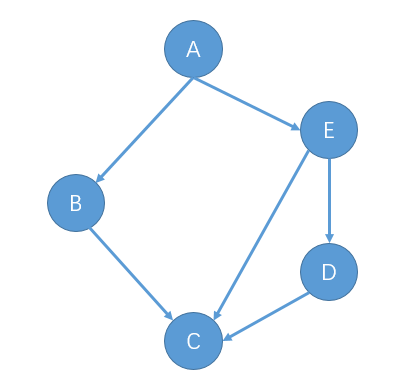
\includegraphics[width=7cm]{structure1.png}
\item \textbf{[5pts]} 请给出下图中按照道德化方法可以找到的所有条件独立的组合(即哪些变量关于哪些变量或者变量集条件独立),独立也算做条件独立的一种特例。

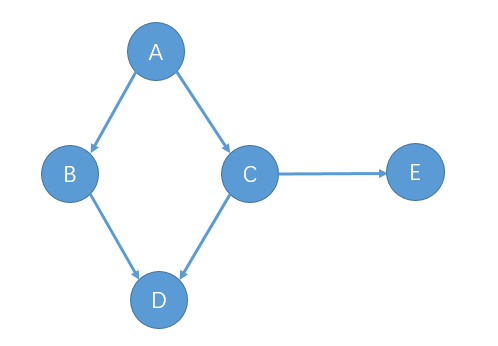
\includegraphics[width=9cm]{structure2.png}


\item \textbf{[10pts]} 在这里,首先我们将给出关于“阻塞”的概念,然后我们根据“阻塞”的概念给出条件独立的充要条件。
\begin{def-box}[阻塞]
设$X,Y,Z$分别是一个有向无环图$G$里互没有交集的结点集,$Z$阻塞$X$中的任一个结点到Y中的任一个结点的通路,当且仅当结点集$Z$满足如下条件:
如果$G$中有顺序结构$x\rightarrow z\rightarrow y$或同父结构$x\leftarrow z\rightarrow y$,则结点$z$包含在集合$Z$中;
如果$G$中有V型结构$x\rightarrow z \leftarrow y$,则结点$z$及其孩子结点一定不包含在集合Z中。
\end{def-box}
\begin{theorem}[条件独立]
\label{theorem}
设$X$和$Y$是{\rm DAG}中的两个结点变量集,$Z$是有向无环图$G$中的不包含$X$和$Y$的结点集合,如果集合$Z$阻塞$X$到$Y$的任何一条道路,则$X$和$Y$在给定$Z$时条件独立,即$X\indep Y|Z$。
\end{theorem}
请根据定理\ref{theorem},判断第一问中有哪些条件独立的组合(独立也算条件独立的一种特例)。

\item \textbf{[10pts]} 由以上两问我们可知,道德化方法中的“除去集合$z$后,$x$和$y$分属两个连通分支”并不构成条件独立性的充要条件。如果对道德化方法稍加修改,在连接V型结构父结点前,我们只保留图中$X,Y,Z$及他们的非孩子结点,之后的步骤则相同。请问你认为用修改后的方法可以保证得到{\color{red}{全部的}}正确的条件独立集合吗?如果可以,请说明理由;如果不能,请给出反例。

\end{enumerate}
\begin{myProof}
	此处用于写证明(中英文均可)
	~\\
	~\\
	~\\
	~\\

\end{myProof}
\newpage
\section{[20pts] Naive Bayes Classifier}
	
	通过对课本的学习,我们了解了采用“属性条件独立性假设”的朴素贝叶斯分类器。现在我们有如下表所示的一个数据集:
	\begin{table}[htp]
		\centering
		\caption{数据集}\label{tab:aStrangeTable}
	\begin{tabular}{c|ccccc}
		\hline 
	编号	& $x_1$ & $x_2$ & $x_3$ & $x_4$ & $y$ \\ 
		\hline 
	样本1	& 1 & 1 & 1 & 0 & 1 \\ 
		\hline 
	样本2	& 1 & 1 & 0 & 0 & 0 \\ 
		\hline 
	样本3	& 0 & 0 & 1 & 1 & 0 \\ 
		\hline 
	样本4	& 1 & 0 & 1 & 1 & 1 \\ 
		\hline 
	样本5	& 0 & 0 & 1 & 1 & 1 \\ 
		\hline 
	\end{tabular}
	\end{table} 
	
	\begin{enumerate}[ {(}1{)}]
		\item \textbf{[10pts]} 试计算:$\Pr\{ y=1 | \mathbf{x}=(1,1,0,1) \}$ 与 $\Pr\{ y=0 | \mathbf{x}=(1,1,0,1) \}$ 的值;
		\item \textbf{[10pts]} 使用“拉普拉斯修正”之后,再重新计算上一问中的值。
	\end{enumerate}
	
\begin{mySol}
	~\\
\begin{enumerate}[ {(}1{)}]
\item 
\begin{equation}
\Pr\{ y=1 | \mathbf{x}=(1,1,0,1) \} = \frac{\Pr\{\mathbf{x}=(1,1,0,1) | y=1  \} \Pr\{y=1\}}{\Pr\{\mathbf{x}=(1,1,0,1) \}}
\end{equation}
根据“属性条件独立性假设”的思想,有:
\begin{equation}
\begin{aligned}
&\Pr\{\mathbf{x}=(1,1,0,1) | y=1  \}\\ 
=& \Pr\{x_1 = 1 | y = 1\}\Pr\{x_2 = 1 | y = 1\}\Pr\{x_3 = 0 | y = 1\}\Pr\{x_4 = 1 | y = 1\}\\
=& \frac{2}{3}\times\frac{1}{3}\times\frac{0}{3}\times\frac{2}{3}\\
=& 0
\end{aligned}
\end{equation}
以及
\begin{equation}
\begin{aligned}
&\Pr\{\mathbf{x}=(1,1,0,1)\}\\ 
=& \Pr\{x_1 = 1\}\Pr\{x_2 = 1\}\Pr\{x_3 = 0\}\Pr\{x_4 = 1\}\\
=& \frac{3}{5}\times\frac{2}{5}\times\frac{1}{5}\times\frac{3}{5}\\
=& \frac{18}{625}
\end{aligned}
\end{equation}
所以可得:
\begin{equation}
\Pr\{ y=1 | \mathbf{x}=(1,1,0,1) \} = 0
\end{equation}
类似的
\begin{equation}
\Pr\{ y=0 | \mathbf{x}=(1,1,0,1) \} = \frac{\Pr\{\mathbf{x}=(1,1,0,1) | y=0  \} \Pr\{y=0\}}{\Pr\{\mathbf{x}=(1,1,0,1) \}}
\end{equation}
根据“属性条件独立性假设”的思想,有:
\begin{equation}
\begin{aligned}
&\Pr\{\mathbf{x}=(1,1,0,1) | y=0  \}\\ 
=& \Pr\{x_1 = 1 | y = 0\}\Pr\{x_2 = 1 | y = 0\}\Pr\{x_3 = 0 | y = 0\}\Pr\{x_4 = 1 | y = 0\}\\
=& \frac{1}{2}\times\frac{1}{2}\times\frac{1}{2}\times\frac{1}{2}\\
=& \frac{1}{16}
\end{aligned}
\end{equation}
以及
\begin{equation}
\Pr\{\mathbf{x}=(1,1,0,1)\} = \frac{18}{625}
\end{equation}
又因为
\begin{equation}
\Pr\{y=0\} = \frac{2}{5}
\end{equation}
综上可得
\begin{equation}
\begin{aligned}
&\Pr\{ y=0 | \mathbf{x}=(1,1,0,1) \}\\ 
=& \frac{\Pr\{\mathbf{x}=(1,1,0,1) | y=0  \} \Pr\{y=0\}}{\Pr\{\mathbf{x}=(1,1,0,1) \}}\\
=& \frac{\frac{1}{16}\times\frac{2}{5}}{\frac{18}{625}}\\ 
=& \frac{125}{144} 
\end{aligned}
\end{equation}

\item 
首先有:
\begin{equation}
\Pr\{\mathbf{x}=(1,1,0,1)\} = \frac{18}{625}
\end{equation}
根据上题,结合“拉普拉斯修正”,可得:
\begin{equation}
\begin{aligned}
&\Pr\{\mathbf{x}=(1,1,0,1) | y=1  \}\\ 
=& \Pr\{x_1 = 1 | y = 1\}\Pr\{x_2 = 1 | y = 1\}\Pr\{x_3 = 0 | y = 1\}\Pr\{x_4 = 1 | y = 1\}\\
=& \frac{3}{5}\times\frac{2}{5}\times\frac{1}{5}\times\frac{3}{5}\\
=& \frac{18}{625}
\end{aligned}
\end{equation}
还有:
\begin{equation}
\Pr\{y=1\} = \frac{4}{7}
\end{equation}
所以得到:
\begin{equation}
\Pr\{ y=1 | \mathbf{x}=(1,1,0,1) \} = \frac{4}{7}
\end{equation}
类似的,根据"拉普拉斯修正",可得:
\begin{equation}
\begin{aligned}
&\Pr\{\mathbf{x}=(1,1,0,1) | y=0  \}\\ 
=& \Pr\{x_1 = 1 | y = 0\}\Pr\{x_2 = 1 | y = 0\}\Pr\{x_3 = 0 | y = 0\}\Pr\{x_4 = 1 | y = 0\}\\
=& \frac{2}{4}\times\frac{2}{4}\times\frac{2}{4}\times\frac{2}{4}\\
=& \frac{1}{16}
\end{aligned}
\end{equation}
还有:
\begin{equation}
\Pr\{y=0\} = \frac{3}{7}
\end{equation}
所以得到:
\begin{equation}
\Pr\{ y=0 | \mathbf{x}=(1,1,0,1) \} = \frac{625}{672}
\end{equation}
\end{enumerate}	

\end{mySol}
\newpage	
\section{[50pts] Ensemble Methods in Practice}

由于出色的性能和良好的鲁棒性,集成学习方法 (Ensemble methods) 成为了极受欢迎的机器学习方法,在各大机器学习比赛中也经常出现集成学习的身影。在本次实验中我们将结合两种经典的集成学习思想:Boosting和Bagging,对集成学习方法进行实践。

本次实验选取UCI数据集Adult,此数据集为一个二分类数据集,具体信息可参照\href{http://archive.ics.uci.edu/ml/datasets/Adult}{链接},为了方便大家使用数据集,已经提前对数据集稍作处理,并划分为训练集和测试集,大家可通过\href{ftp://lamda.nju.edu.cn/ml2018/PS5/adult_dataset.zip}{此链接}进行下载。

由于Adult是一个类别不平衡数据集,本次实验选用AUC作为评价分类器性能的评价指标,AUC指标的计算可调用\href{http://scikit-learn.org/stable/modules/generated/sklearn.metrics.roc_auc_score.html}{sklearn算法包}。

\begin{enumerate}[(1)]
	\item \textbf{[5pts]} 本次实验要求使用Python 3或者Matlab编写,要求代码分布于两个文件中,BoostMain.py、RandomForestMain.py (Python) 或 BoostMain.m、RandomForestMain.m (Matlab),调用这两个文件就能完成一次所实现分类器的训练和测试;
	
	\item \textbf{[35pts]} 本次实验要求编程实现如下功能:
	
	\begin{itemize}
		\item \textbf{[10pts]} 结合教材8.2节中图8.3所示的算法伪代码实现AdaBoost算法,基分类器选用决策树,基分类器可调用sklearn中\href{http://scikit-learn.org/stable/modules/generated/sklearn.tree.DecisionTreeClassifier.html}{决策树}的实现;
		\item \textbf{[10pts]} 结合教材8.3.2节所述,实现随机森林算法,基分类器仍可调用sklearn中决策树的实现,当然也可以自行手动实现,在实验报告中请给出随机森林的算法伪代码;
		\item \textbf{[10pts]} 结合AdaBoost和随机森林的实现,调查基学习器数量对分类器训练效果的影响 (参数调查),具体操作如下:分别对AdaBoost和随机森林,给定基分类器数目,在训练数据集上用5折交叉验证得到验证AUC评价。在实验报告中用折线图的形式报告实验结果,折线图横轴为基分类器数目,纵轴为AUC指标,图中有两条线分别对应AdaBoost和随机森林,基分类器数目选取范围请自行决定;
		\item \textbf{[5pts]} 根据参数调查结果,对AdaBoost和随机森林选取最好的基分类器数目,在训练数据集上进行训练,在实验报告中报告在测试集上的AUC指标;
	\end{itemize}
	
	\item \textbf{[10pts]} 在实验报告中,除了报告上述要求报告的内容外还需要展现实验过程,实验报告需要有层次和条理性,能让读者仅通过实验报告便能了解实验的目的,过程和结果。
	
\end{enumerate}

\noindent{\textbf{实验报告.}}
	
\end{document}